
%(BEGIN_QUESTION)
% Copyright 2007, Tony R. Kuphaldt, released under the Creative Commons Attribution License (v 1.0)
% This means you may do almost anything with this work of mine, so long as you give me proper credit

This metal-melting furnace has a cascade control system, whereby a ``bath'' controller (sensing the temperature of the molten metal) acts as the primary, and a ``crown'' controller (sensing the temperature of the refractory wall and roof) acts as the secondary.  The burner's heat output is a direct function of air flow through it; therefore, a wider-open air valve causes a more intense fire from the burner:

$$\includegraphics[width=15.5cm]{i01826x01.eps}$$

Sometimes a thick layer of ``slag'' covers the surface of the metal, impeding heat transfer from the burner flame to the molten metal bath.  The bath controller, sensing low metal temperature, sends an ever-increasing setpoint to the crown controller, raising the air temperature inside the furnace to high levels, which then shortens the life of the refractory brick.

Can you think of a solution to this problem, whereby the secondary control loop won't be driven into saturation in the event of slag on the metal surface?

\vskip 20pt \vbox{\hrule \hbox{\strut \vrule{} {\bf Suggestions for Socratic discussion} \vrule} \hrule}

\begin{itemize}
\item{} Why do you suppose this furnace is equipped with a cascade control system at all?  What would be wrong with just a simple single-loop PID control of metal temperature?
\end{itemize}

\underbar{file i01826}
%(END_QUESTION)





%(BEGIN_ANSWER)

%(END_ANSWER)





%(BEGIN_NOTES)

The high-limit function prevents crown overheating, while the high differential temperature alarm informs operators of a slag problem:

$$\includegraphics[width=15.5cm]{i01826x02.eps}$$









\vskip 20pt \vbox{\hrule \hbox{\strut \vrule{} {\bf Virtual Troubleshooting} \vrule} \hrule}

This question is a good candidate for a ``Virtual Troubleshooting'' exercise.  Presenting the diagram to students, you first imagine in your own mind a particular fault in the system.  Then, you present one or more symptoms of that fault (something noticeable by an operator or other user of the system).  Students then propose various diagnostic tests to perform on this system to identify the nature and location of the fault, as though they were technicians trying to troubleshoot the problem.  Your job is to tell them what the result(s) would be for each of the proposed diagnostic tests, documenting those results where all the students can see.

During and after the exercise, it is good to ask students follow-up questions such as:

\begin{itemize}
\item{} What does the result of the last diagnostic test tell you about the fault?
\item{} Suppose the results of the last diagnostic test were different.  What then would that result tell you about the fault?
\item{} Is the last diagnostic test the best one we could do?
\item{} What would be the ideal order of tests, to diagnose the problem in as few steps as possible?
\end{itemize}


%INDEX% Control, strategies: cascade with limits
%INDEX% Process: combustion furnace

%(END_NOTES)


